\documentclass[14pt,fleqn]{extarticle}
\RequirePackage{prepwell}
\previewoff
\begin{document}

\newcommand\ea{100-x^2}
\newcommand\es{\sqrt{\ea}}
\newcommand\eb{\left(x+10 \right)}

%text
If the length of three sides of trapezium 
other than the base is 10cm each, find the 
area of the trapezium when it is maximum
%

\newcard

%text
You can have \underline{infinite} quadrilaterals with
three sides equal to $10$ cm\newline 

But you can have
\underline{only one} trapezium (with $PS\parallel QR$) that has 
three sides equal \newline 

Moreover, in the figure below 
\begin{center} 
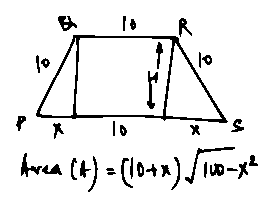
\includegraphics[scale=1.5]{figure.eps} 
\end{center} 
\begin{align}
\text{Height } H &= \sqrt{10^2 - x^2} = \sqrt{100-x^2} \\
\therefore A &= \frac{1}{2}\cdot \left(QR + PS \right)\cdot H \\
&= \frac{1}{2}\cdot \left(10 + 10 +2x \right)\cdot \sqrt{100-x^2} \\
&= \left(10+x \right)\cdot \sqrt{100-x^2} 
\end{align}

\newcard

\begin{align}
	\frac{dA}{dx} &= - \frac{2\cdot \left(x^2 + 5x-50 \right)}{\es} \\
	\therefore \frac{dA}{dx} &=0 \implies x = 5 
\end{align}

\newcard 

Given that $A = \eb\cdot\es$

\begin{align}
\frac{dA}{dx} &= \overbrace{\es \frac{d}{dx}\eb + \eb \frac{d}{dx}\es}^{\text{Product Rule}} \\
&= \es + \frac{\eb}{2\cdot \es}\cdot \left(-2x \right) \\
&= \frac{\ea - \left\lbrace x\cdot \eb\right\rbrace}{\es} \\
&= -\frac{2\cdot \left(x^2+5x-50 \right)}{\es} = - \frac{2\cdot (x-5)\cdot (x+10)}{\es} \\
\therefore \frac{dA}{dx} &= 0 \implies (x-5)\cdot (x+10) = 0 \\
\text{or } x &= 5, -10\text{ (non-sensical)}
\end{align} 

Hence $A$ has an \underline{extreme value} when $x=5$

\newcard 

\[ \frac{d^2 A}{dx^2} = -2\sqrt{3} \text{ when } x = 5 \]
And the maximum area $A_m = 75\sqrt{3}$ units 

\newcard 

\[ \frac{d^2 A}{dx^2} = -\sqrt{3} \text{ when } x = 5 \]
And the maximum area $A_m = 75\sqrt{3}$ units 

\newcard 


Let $g(x) = x^2 + 5x - 50$\newline 

\begin{align}
\frac{dA}{dx} &= -\frac{2\cdot g(x)}{\es}\\
\therefore \frac{d^2 A	}{dx^2} &= -2 \underbrace{\left[\frac{\es \cdot g'(x) - g(x) \frac{d}{dx}\es}{\left(\es \right)^2} \right]}_{\text{Quotient Rule}}
\end{align}

Now, recall that $g(x) = x^2 + 5x-50 = 0$ for $x = 5$, that is $g(5) = 0$. Hence 

\begin{align}
\left[ \frac{d^2 A}{dx^2}\right]_{x=5} &= -2 \left[\frac{\es\cdot g'(x)}{\ea} \right]_{x=5}\\
\text{where } g'(x) &= 2x + 5 \\ 
\therefore \left[ \frac{d^2 A}{dx^2}\right]_{x=5} &= -2 \left[\frac{\sqrt{100-5^2}\cdot (10 + 5)}{100 - 5^2}\right] \\
&= -\frac{30}{\sqrt{75}} = -\frac{6}{\sqrt{3}} = -2\sqrt{3} 
\end{align}

And as $\dfrac{d^2A}{dx^2} < 0$ at $x=5$, therefore we have a \underline{maxima} at $x=5$ 

And the \underline{maximum area} is  
\[ A_m = (10+5)\cdot \sqrt{100-5^2} = 75\sqrt{3}\text{ sq. units}\]

\end{document}